% Project Specifications
%\clearpage%if the chapter heading starts close to bottom of the page, force a line break and remove the vertical vspace
\vspace{21.5pt}
\chapter{Implementation}
\section{Software  setup}

First state of project was getting initial programming environment ready, consisting of rp2040 SDK, GCC crosscompiler and visual studio code with plugins [insert here] and a j-link debugger to program and debug on the MCU, and a logic analyser to help monitor the debug traffic for verification.

\section{Hardware setup}

\begin{figure}[ht]
	\centering
	\AltText{Initial POC hardware setup showing direct soldered wiring between J-Link Edu and a Raspberry pi Pico}{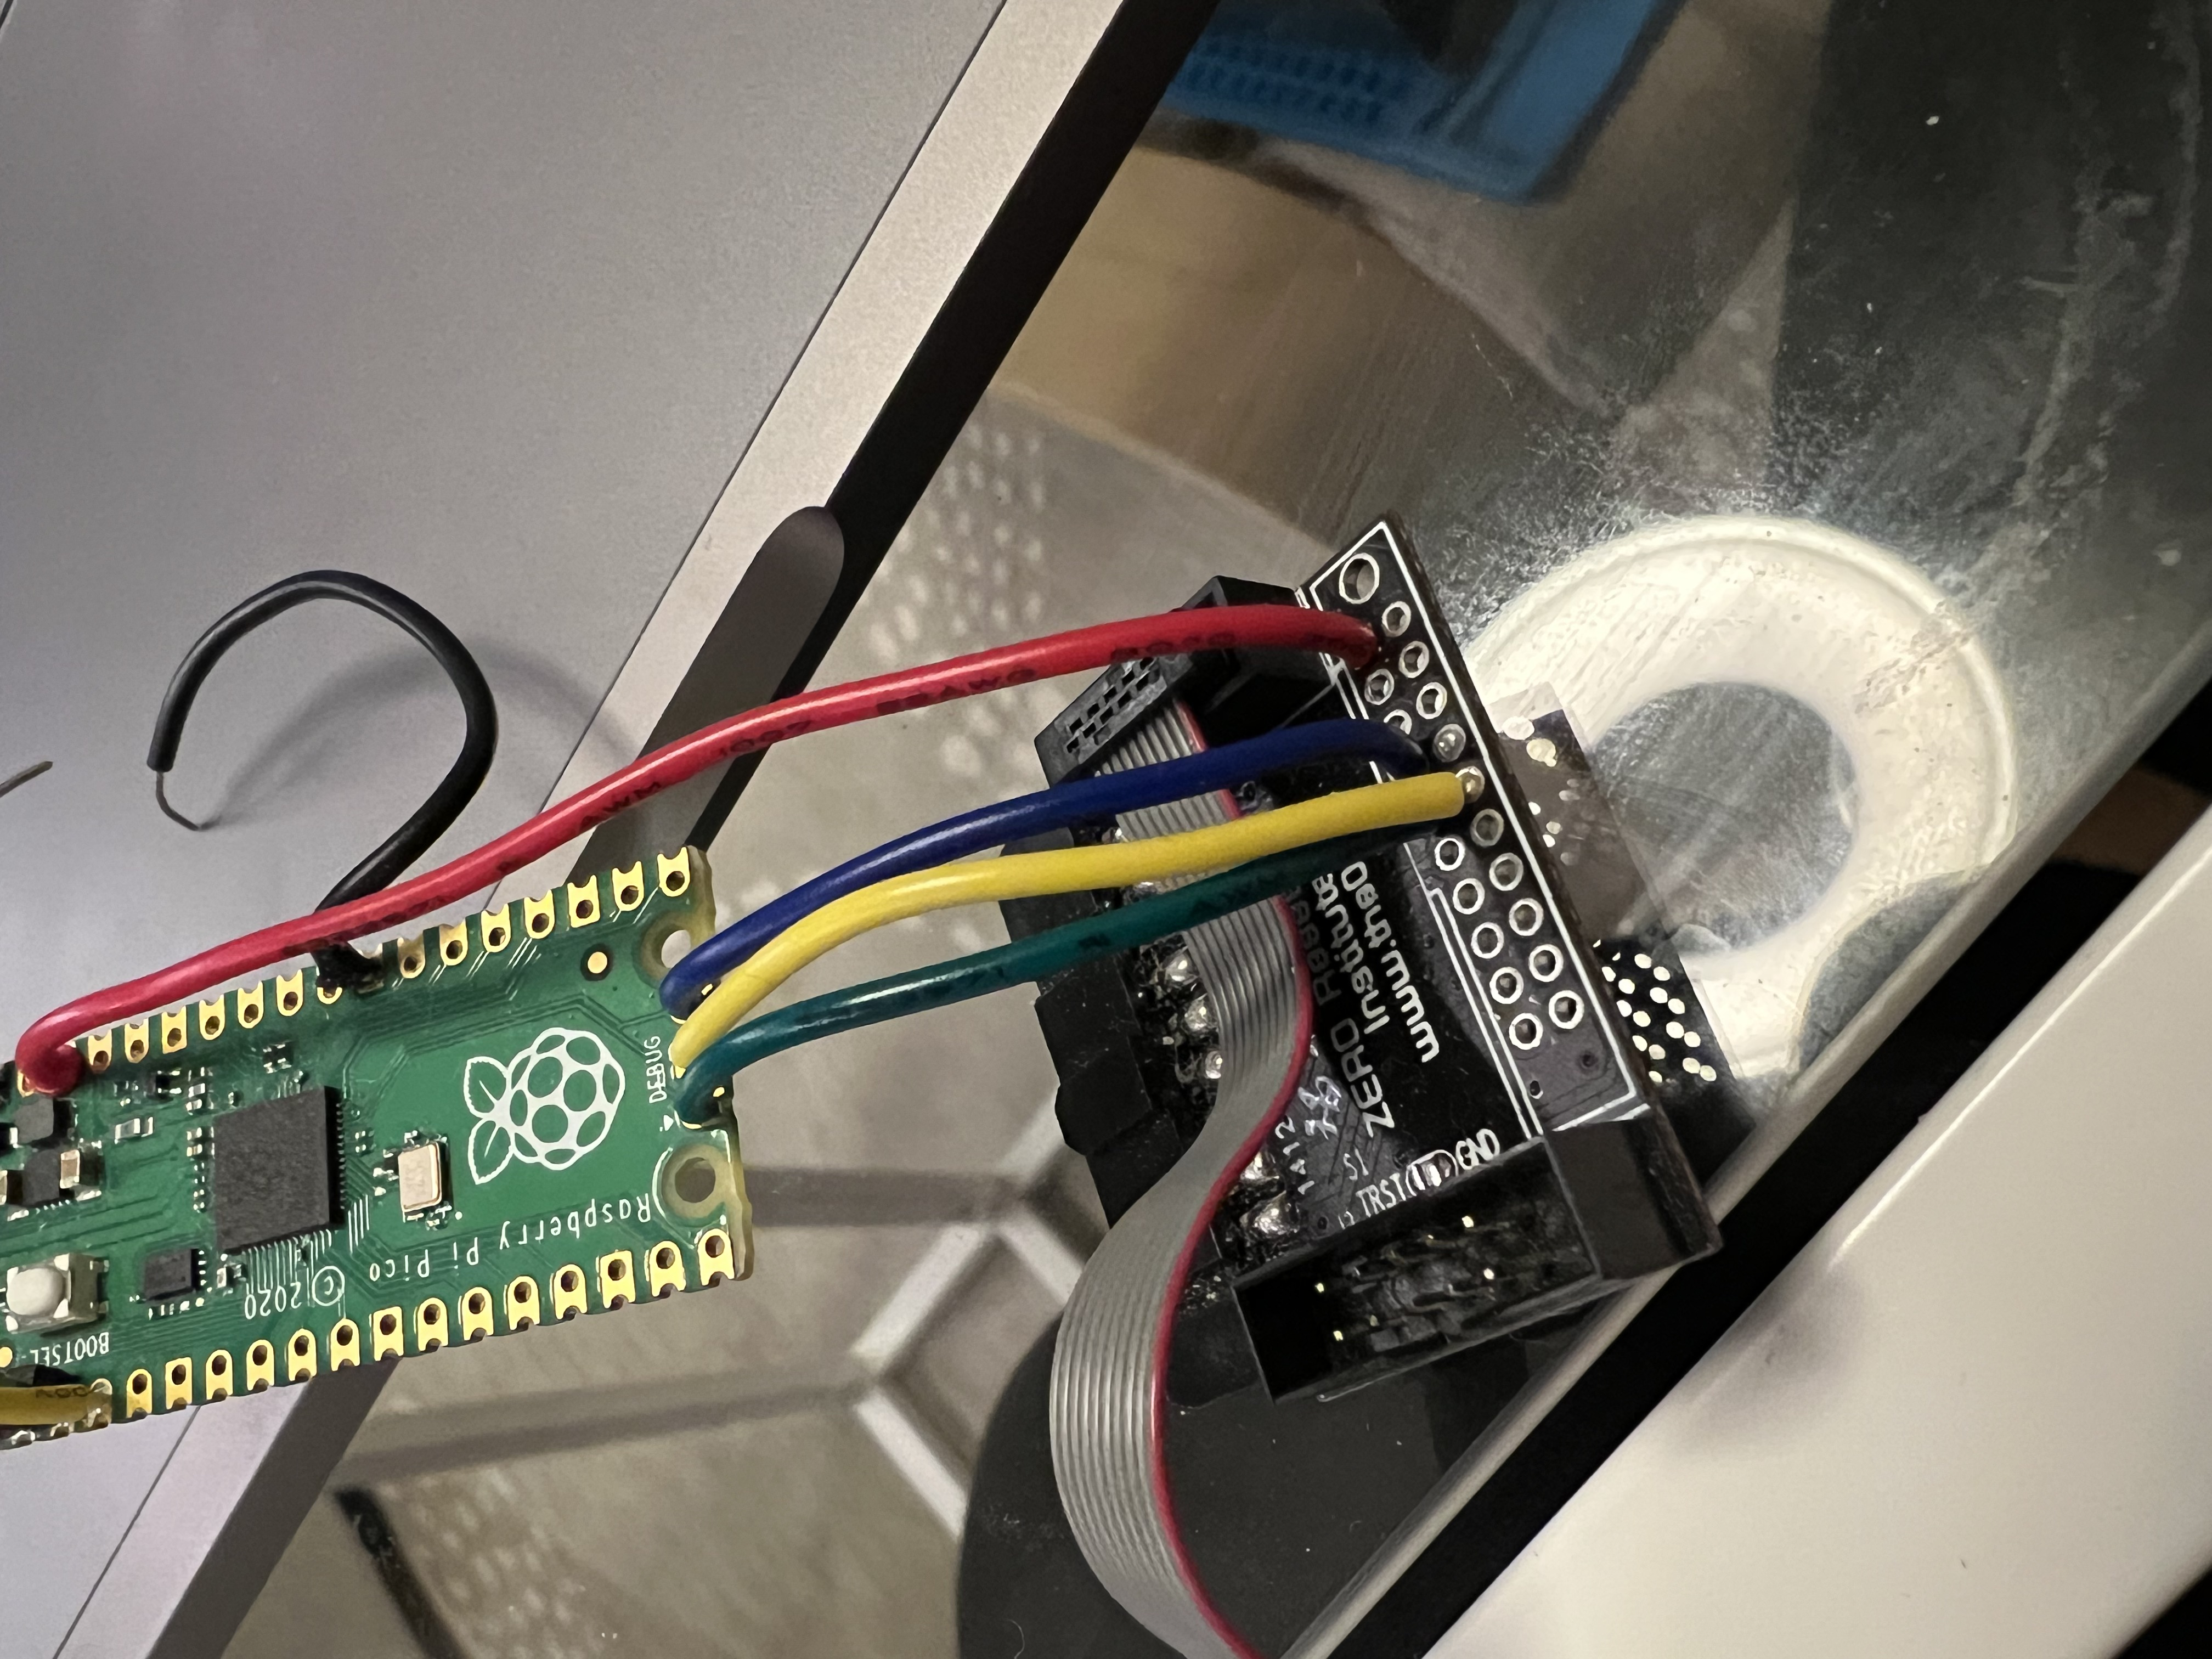
\includegraphics[width=\textwidth]{initial POC setup}}
	\caption{initial POC setup}
	\label{fig:InitialPOCwiring}
\end{figure}

For initial proof of concept a Pi Pico was directly wired into a jlink debugger wth directly soldered wires for simplicity as show in \ref{fig:InitialPOCwiring}.

A jumper cable is used to simulate closing of a mounting interface interlock.

\pagebreak
\begin{figure}[ht]
	\centering
	\AltText{Full POC hardware setup showing display and buttons for UI on breadboads along with target device}{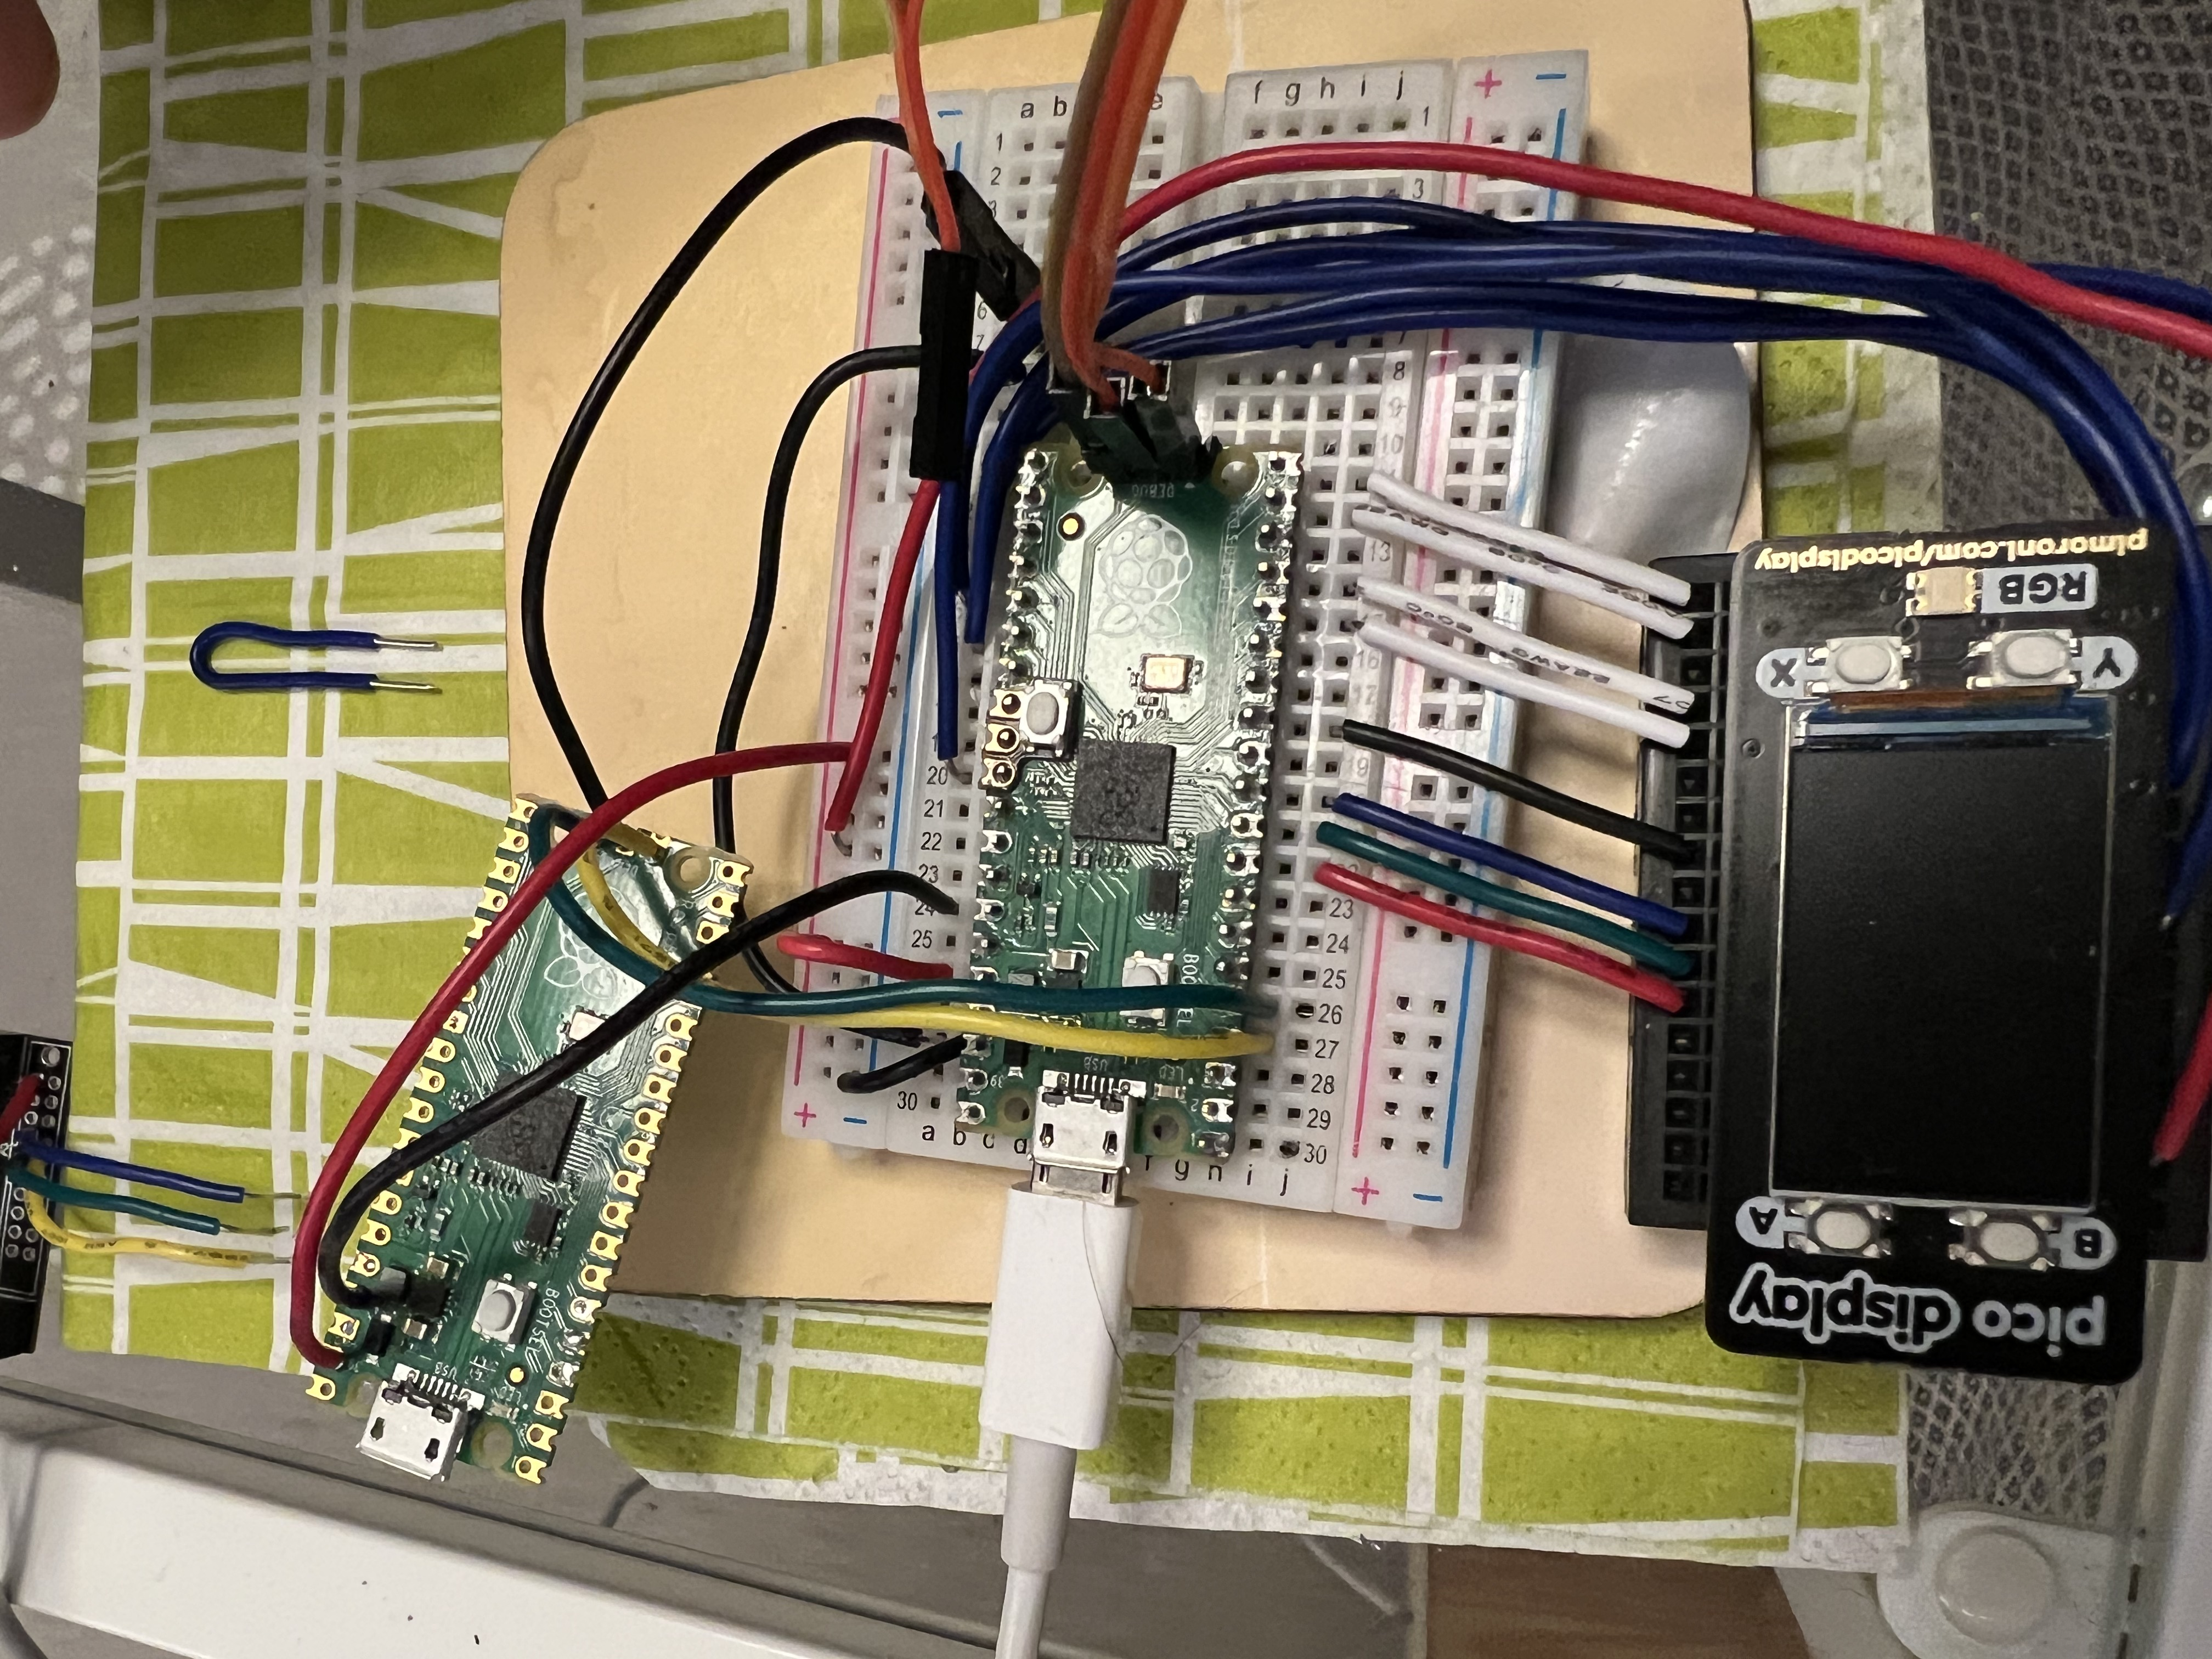
\includegraphics[width=\textwidth]{full POC setup}}
	\caption{Full wiring on breadboard with Interface}
	\label{fig:FullPOCwiring}
\end{figure}

This was later expanded to include a Pimoroni display and buttons for a user interface, and second Pi Pico as flashing target \ref{fig:FullPOCwiring}.

\section{Software bootstrap}

Initial step was to establish SWD setup as lowest level critical component, this took longer than anticipated after initial response reading DPIDR succeeded to verify an ARM debug unit was reponding, but further attempted operations such as memory read failed. Reason for failure transpired to a lack of accounting multiple debug units\cite{RaspberryPiPico} with many references to SWD implementation omitting the step of device selection from the setup sequence owing to most ARM MCU's only having one core this being an uncessary step.

Once handshake was established the most critical functions of memory write and read were implemented and verified to confirm successful control over SWD, 

From there a small RAM resident test program to blink the onboard LED was created as a test case binary to to be writte and executed from memory via SWD for a simple control verification.

Programming sequence detailed description can be found in Appendix 1.


Picture of loading UI

Picture of flashing operation

